%%%%%%%%%%%%%%%%%%%%%%%%%%%%%%%%%%%%%%%%%%%%%%%%%%%%%%%%%%%%%%%%%%%%%%%%%%%%%%%%
% AMS Beamer series / Bologna FC / Template
% Andrea Omicini
% Alma Mater Studiorum - Università di Bologna
% mailto:andrea.omicini@unibo.it
%%%%%%%%%%%%%%%%%%%%%%%%%%%%%%%%%%%%%%%%%%%%%%%%%%%%%%%%%%%%%%%%%%%%%%%%%%%%%%%%
%\documentclass[handout]{beamer}\mode<handout>{\usetheme{default}}
%
\documentclass[presentation, 9pt, aspectratio=169]{beamer}\mode<presentation>{\usetheme{AMSBolognaFC}}
%\documentclass[handout]{beamer}\mode<handout>{\usetheme{AMSBolognaFC}}
%%%%%%%%%%%%%%%%%%%%%%%%%%%%%%%%%%%%%%%%%%%%%%%%%%%%%%%%%%%%%%%%%%%%%%%%%%%%%%%%
\usepackage[T1]{fontenc}
\usepackage{wasysym}
\usepackage{amsmath,blkarray}
\usepackage{soul}
\usepackage[minted,most]{tcolorbox}
\usepackage{centernot}
\usepackage{fontawesome}
\usepackage{fancyvrb}
\usepackage{minted}
\usepackage{hyperref}
\usepackage{multicol}
\setminted[scala]{fontsize=\small,frame=lines,baselinestretch=1,obeytabs=true, tabsize=2}
\setminted[yaml]{fontsize=\large,frame=lines,linenos,baselinestretch=1,obeytabs=true, tabsize=2}
\usepackage[ddmmyyyy]{datetime}
\setminted{fontsize=\footnotesize}
\renewcommand{\dateseparator}{}
%\renewcommand{\thefootnote}{\fnsymbol{footnote}}
\newcommand{\version}{1}

\usepackage[
	%backend=biber,
	backend=bibtex,
%	citestyle=authoryear-icomp,
%	maxcitenames=1,
	style=alphabetic]{biblatex}

	\makeatletter

%\addbibresource{biblio.bib}

\bibliography{biblio}

\newcommand\extrafootertext[1]{%
    \bgroup
    \renewcommand\thefootnote{\fnsymbol{footnote}}%
    \renewcommand\thempfootnote{\fnsymbol{mpfootnote}}%
    \footnotetext[0]{#1}%
    \egroup
}

\newcommand{\citeinslide}[1]{\cite{#1}\extrafootertext{\scriptsize\cite{#1} \fullcite{#1}}}


%%%%%%%%%%%%%%%%%%%%%%%%%%%%%%%%%%%%%%%%%%%%%%%%%%%%%%%%%%%%%%%%%%%%%%%%%%%%%%%%
\title[A Soft-Eng Approach for CPSWs!]
{A Language-based Software Engineering Approach for Cyber-Physical Swarms}
%
%
\author[\sspeaker{G.Aguzzi}]
{\speaker{Gianluca Aguzzi} \href{mailto:gianluca.aguzzi@unibo.it}{gianluca.aguzzi@unibo.it} \\
\textbf{Supervisor:} \speaker{Mirko Viroli} \href{mailto:mirko.viroli@unibo.it}{mirko.viroli@unibo.it}}
%
\institute[DISI, Univ.\ Bologna]
{%Dipartimento di Informatica -- Scienza e Ingegneria (DISI)\\
\textsc{Alma Mater Studiorum} -- Universit{\`a} di Bologna \\[0.1cm]
\textbf{Final Year PhD Report}\\[0.15cm]
}
%
\renewcommand{\dateseparator}{/}
\date[\today]{\today}
%
\AtBeginSubsection[]
{
  \begin{frame}
  \frametitle{Contents}
  \tableofcontents[currentsubsection, 
	sectionstyle=show/shaded, 
	subsectionstyle=show/shaded]
  \end{frame}
}
\AtBeginSection[]
{
  \begin{frame}
  \frametitle{Contents}
  \tableofcontents[currentsubsection, 
	sectionstyle=show/shaded, 
	subsectionstyle=show/shaded]
  \end{frame}
}
%%%%%%%%%%%%%%%%%%%%%%%%%%%%%%%%%%%%%%%%%%%%%%%%%%%%%%%%%%%%%%%%%%%%%%%%%%%%%%%%

\lstdefinelanguage{scala}{
  keywords={abstract,case,catch,class,def,%
    do,else,extends,false,final,finally,%
    for,if,implicit,import,match,mixin,%
    new,null,object,override,package,%
    private,protected,requires,return,sealed,%
    super,this,throw,trait,true,try,lazy,%
    type,val,var,while,with,yield,forSome},
  otherkeywords={=>,<-,<\%,<:,>:,\#},
  sensitive=true,
  morecomment=[l]{//},
  morecomment=[n]{/*}{*/},
  morestring=[b]",
  morestring=[b]',
  morestring=[b]""",
  basicstyle=\lst@ifdisplaystyle\footnotesize\fi\ttfamily,
  emphstyle=\bfseries
}
\definecolor{ddarkgreen}{rgb}{0,0.5,0}
\lstdefinelanguage{scafi}{frame=single,basewidth=0.5em,language={scala},
keywordstyle=\color{blue}\textbf, commentstyle=\color{ddarkgreen},
keywordstyle=[2]\color{red}\textbf, keywords=[2]{rep,nbr,foldhood,foldhoodPlus,aggregate,branch,spawn},
keywordstyle=[3]\color{gray}, keywords=[3]{Me,AroundMe,Everywhere,Forever}, %,@@,@@@
keywordstyle=[4]\color{red}\textbf, keywords=[4]{in,out,rd},
keywordstyle=[5]\color{violet}, keywords=[5]{evolve,when,andNext,workflow,C,gossip},
keywordstyle=[6]\color{orange}, keywords=[6]{Available,Serving,Done,Waiting,Removing}}

\newcommand{\hsplit}[2]{
\begin{minipage}{0.48\textwidth}
#1
\end{minipage}
\hfill
\begin{minipage}{0.48\textwidth}
#2
\end{minipage}
}
\newcommand{\hsplits}[4]{
\begin{minipage}{#1\textwidth}
#3
\end{minipage}
\hfill
\begin{minipage}{#2\textwidth}
#4
\end{minipage}
}

\newcommand{\lbl}[1]{\textbf{\textcolor{gray!90!white}{#1}}}
\newcommand{\enf}[1]{{\textcolor{red}{#1}}}
\newcommand{\bo}[1]{\textbf{#1}}

\newcommand{\imgh}[2]{
\begin{figure}
\centering
\includegraphics[width=#1\textwidth]{img/#2}
\end{figure}
}
\newcommand{\imgv}[2]{
\begin{figure}
\centering
\includegraphics[height=#1\textheight]{img/#2}
\end{figure}
}

\newtcblisting{mycode}[3]{%
  boxsep=0pt,
  boxrule=0pt,
  arc=1mm, 
  left=1mm,
  %auto outer arc,
  size=fbox,%tight,
  %colframe=blue!40!black, colframe=black!30!white,
  %colbacktitle=blue!80!white,
  colback=blue!5,
  %toprule=0.1mm, bottomrule=0.1mm, rightrule=0.1mm, leftrule=1mm, 
  listing only,
  listing options={language=scafi, alsoletter={-},
    backgroundcolor={},
  	columns=fullflexible,
  	lineskip={-1.5pt},
  	xleftmargin=0px,
  	belowskip={0px},
  	aboveskip={0px},
  	frame=none,
  	#2
  },
  title={#3},#1
}
\lstdefinestyle{s}{basicstyle=\ttfamily\footnotesize}
\lstdefinestyle{ss}{basicstyle=\ttfamily\scriptsize}
\lstdefinestyle{sss}{basicstyle=\ttfamily\tiny}
\lstdefinestyle{conf}{language={},morecomment=[l][\color{darkgreen}]{\#},
basicstyle=\ttfamily\scriptsize}

\newcommand{\question}[1]{\textcolor{darkgray}{\emph{\bo{#1}}}}
\newcommand{\refslide}[1]{Slide~\ref{#1}}

\begin{document}
%%%%%%%%%%%%%%%%%%%%%%%%%%%%%%%%%%%%%%%%%%%%%%%%%%%%%%%%%%%%%%%%%%%%%%%%%%%%%%%%

%/////////
\frame{\titlepage}
%/////////

%===============================================================================
\section*{\refname}
%===============================================================================

%%%%
%/////////
\begin{frame}
\centering
\bold{\Huge{Cyber-Physical Swarms (CPSW)}}
\begin{multicols}{3}
	\begin{figure}
		\large{Many \bold{networked} agents}\\[0.1cm]
		\includegraphics[width=0.3\textwidth]{example-image-a}
	\end{figure}
	\begin{figure}
		\large{Cyber-physical systems}\\[0.1cm]
		\includegraphics[width=0.3\textwidth]{example-image-b}
	\end{figure}
	\begin{figure}
		\large{\bold{Collective} intelligence}\\[0.1cm]
		\includegraphics[width=0.3\textwidth]{example-image-c}
	\end{figure}
\end{multicols}
\end{frame}

\begin{frame}{Context -- Cont.}
\begin{alertblock}{Applications}
  \begin{multicols}{3}
    \begin{itemize}
      \item Swarm robotics
      \item Crowd of (augmented) people
      \item Large-scale IoT systems
      \item Smart cities
      \item COMMunity-OrieNted WEARrable Computing Systems (PRIN project)
    \end{itemize}
  \end{multicols}
\end{alertblock}

\begin{exampleblock}{Challenges}
  \begin{multicols}{3}
    \begin{itemize}
      \item (Unwanted) Emergents
      \item Local to global mapping
      \item Scale
      \item Failures
      \item Distributed control
      \item Complex \& layered architectures
    \end{itemize}
  \end{multicols}
\end{exampleblock}
\centering
\vspace{0.5 cm}
\only<2>{\bold{\huge{How to engineer such applications?}}}
\end{frame}
\begin{frame}{Context -- Cont.}
  \begin{alertblock}{Thesis goal}
    Finds a \emph{systematic} methodology to \bold{synthesize} and \bold{deploy} \emph{\underline{self-organising}} behaviours of \bold{predictable} outcomes
  \end{alertblock}
  \begin{exampleblock}{Multi-Faceted scientific problem}
    \begin{itemize}
      \item \bold{how} to express collective behaviours (algorithms \& methodologies)
      \item \bold{how} to execute specific behaviours (execution models \& middleware dynamics)
      \item \bold{how} to deploy the computation \emph{\underline{smartly}} (deployment)      
    \end{itemize}
  \end{exampleblock}
  \begin{alertblock}{State-of-the art}
    \begin{itemize}
      \item Manual design
      \begin{itemize}
        \item Programming languages with primitives and \emph{collective} abstractions for CPSW (e.g., \emph{\underline{aggregate programming}})
        \item {\bold{\faThumbsUp}} Declarative \& modular \lbl{\faThumbsDown} Limited adaptability w.r.t., non-stationary envs, high knowledge requirements 
      \end{itemize}
      \item Automatic design
      \begin{itemize}
        \item Machine learning methodologies for synthesize collective  behaviours (e.g., \emph{\underline{multi-agent reinforcement learning}})
        \item {\bold{\faThumbsUp}} Learn by doing \lbl{\faThumbsDown} Black-box, not predictable 
      \end{itemize}
    \end{itemize}
  \end{alertblock}
\end{frame}

\begin{frame}{Contribution -- One slide}
\centering{\huge{Models, tools, and algorithms are built around a \emph{\underline{programming language}}}}
\\[0.5cm]
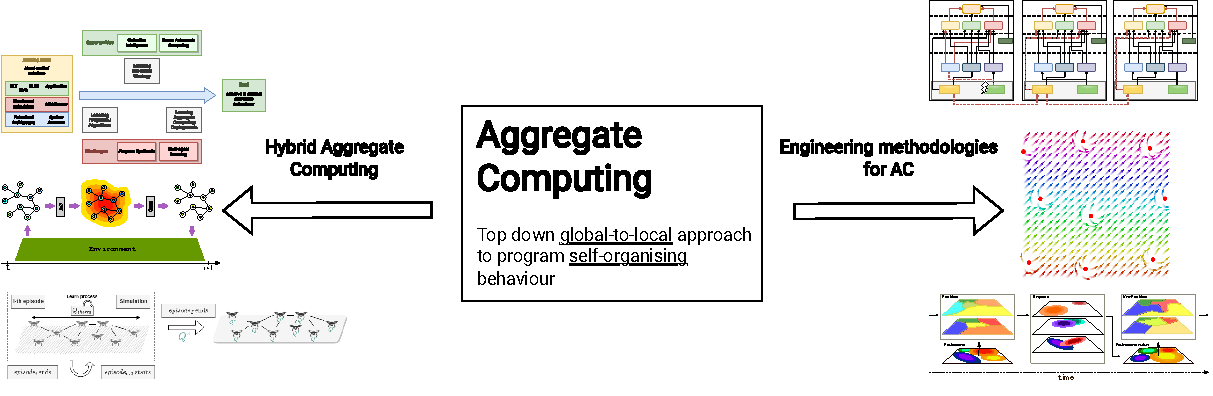
\includegraphics[width=\textwidth]{img/contribution.drawio.pdf}
\end{frame}
\begin{frame}{Aggregate Computing -- One slide}
  \hsplit{

  \begin{block}{\footnotesize Self-org-like computational model}
  \scriptsize
  
  \lbl{interaction:} \emph{repeated} msg exchange with \bo{neighbours}\vspace{0.1cm}
  
  \lbl{behaviour:} \emph{repeated} execution of \enf{async rounds} of \bo{sense -- compute -- (inter)act} \vspace{0.1cm}
  
  
  \lbl{formal model of executions:} event structures \vspace{0.1cm}
  
  %\lbl{semantics:} (1) device; (2) network; (3) global comp.
  \end{block}
  
  %\uncover<3-4>{
  \begin{block}{}
  \scriptsize
  
  \lbl{abstraction:} \bo{computational fields} ($\mathit{dev/evt} \mapsto \mathbb{V}$) \vspace{0.1cm}
  
  \lbl{formal core language:} field calculus~\cite{vbdacp:ac:survey:jlamp}\vspace{0.1cm}
  
  \lbl{paradigm:} \bo{functional, macro-programming} \vspace{0.1cm} %--- supporting compositionality
  
  \centering
  \imgv{0.22}{channel.pdf}
  \end{block}
  
  \tiny \fullcite{vbdacp:ac:survey:jlamp}%\fullcite{beal2015aggregate-programming}
  
  %}
  }{
  
  %\uncover<2-4>{
  \begin{block}{\footnotesize Why?}
    \scriptsize
    
    {\bold{\faThumbsUp}} \, Decouple the collective specification from the IT networks  \vspace{0.1cm}
    
    {\bold{\faThumbsUp}} \, Scale naturally with nodes in the systems  \vspace{0.1cm}
     
    {\bold{\faThumbsUp}} \, High-level abstractions to devise applications
    
    %\lbl{semantics:} (1) device; (2) network; (3) global comp.
  \end{block}
  %}
  
  %\uncover<4-4>{
  \begin{block}{} %{Engineering approach}
  \imgv{0.32}{layerss.pdf}
  \tiny \fullcite{bpv:aggregate:programming}
  \end{block}
  %}
  }
  
\end{frame}
\begin{frame}{Hybrid Aggregate computing}
\vspace{-0.5cm}
\begin{columns}[t]
\begin{column}{0.31\textwidth}
\begin{exampleblock}{Research roadmap~\cite{DBLP:conf/icdcs/AguzziCV22}}
  \footnotesize{
  Highlights goals:
\begin{itemize}
  \item \underline{functionality} (e.g., a certain collective behaviour)
  \item \underline{non-functionality} (e.g., energy consumption)
\end{itemize}}
and means:
\begin{itemize}
  \item \underline{algorithms}
  \item \underline{execution strategy}
  \item \underline{system structures}
\end{itemize}
  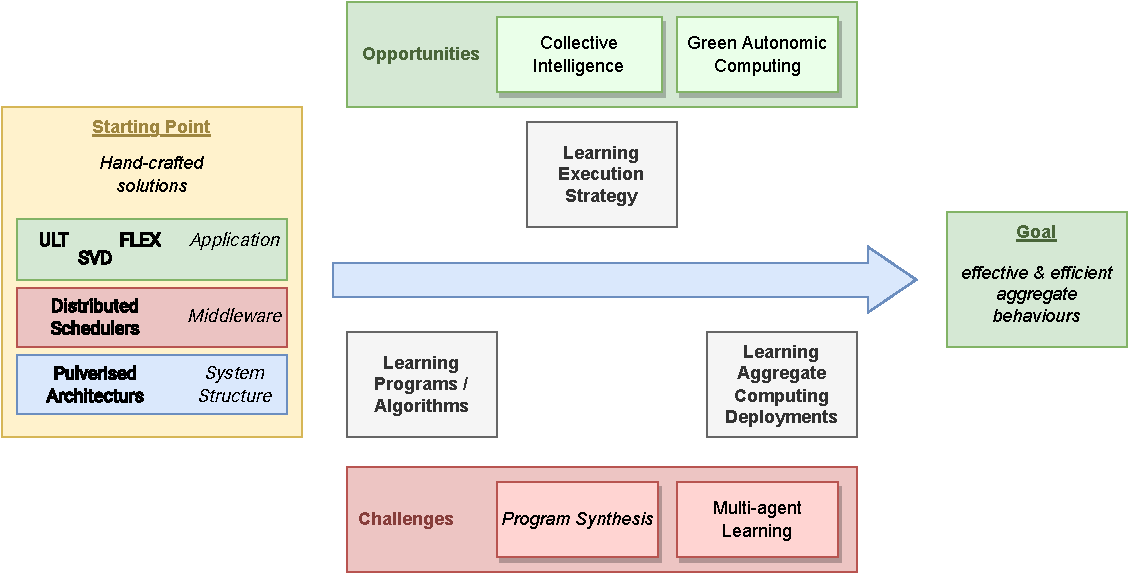
\includegraphics[width=\textwidth]{img/roadmap.pdf}
\end{exampleblock}
\end{column}

\begin{column}{0.31\textwidth}
\begin{exampleblock}{Collective Program Sketching~\cite{DBLP:conf/coordination/AguzziCV22}}
  \footnotesize{
  %% breaks the above sentence in itemize:
  \begin{itemize}
    \item \emph{\underline{holes}}: \emph{\underline{blocks}} of the aggregate program depending on \emph{\underline{environment dynamics}}
    \item \emph{\underline{sketching}}: \emph{\underline{partial}} specification of the aggregate program
    \item Idea: \emph{\underline{synthesis}} of the \emph{\underline{holes}} by \emph{\underline{learning}} from the \emph{\underline{realistic simulation}}
  \end{itemize}}
  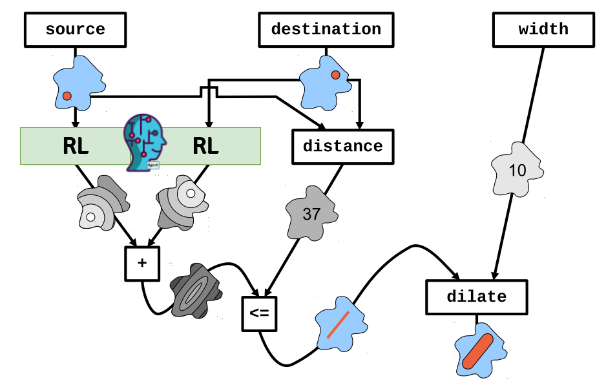
\includegraphics[width=\textwidth]{img/synthesis-3.png}
\end{exampleblock}
\end{column}
\begin{column}{0.31\textwidth}
\begin{exampleblock}{Distributed schedulers~\cite{DBLP:conf/acsos/AguzziCV22}}
  \footnotesize{
  \begin{itemize}
    \item The aggregete computing model does not \underline{enforce} a global-synchronization
    \item \emph{\underline{Distributed}} schedulers: \emph{\underline{local}} decisions on the \emph{\underline{rounds}} of the aggregate program
    \item Idea: \emph{\underline{learning}} the \emph{\underline{best}} scheduling strategy directly by-doing
  \end{itemize}
  }
  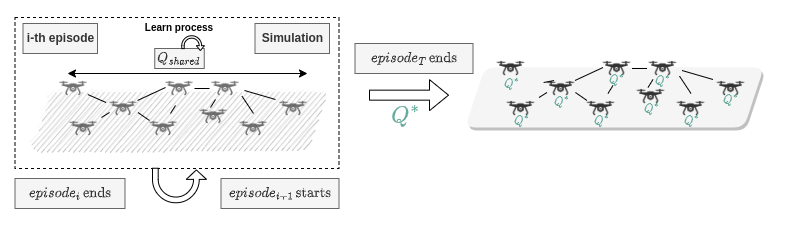
\includegraphics[width=\textwidth]{img/algorithm-learning.png}
\end{exampleblock}
\end{column}  
\end{columns}
\end{frame}

\begin{frame}{Hybrid Aggregate computing -- Cont.}
  
\begin{exampleblock}{Field-Informed reinforcement learning~\cite{acgnn}}
  \begin{itemize}
    \item Aggregate computing is used to \emph{\underline{inform}} the learning process
    \begin{itemize}
      \item Speeding up the training \& Reducing the search space
    \end{itemize} 
    \item Field used as a way to produce a stygmertic representation of the environment
    \item Learning performed through \emph{\underline{deep reinforcement learning}}
    \item Graph-neural networks used as a policy function approximator
  \end{itemize}
\centering
  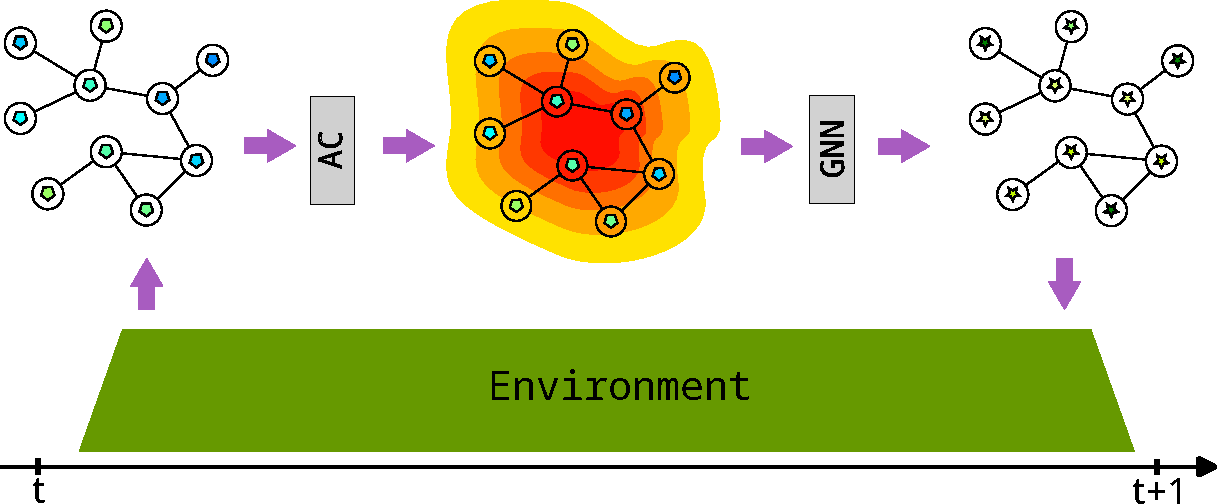
\includegraphics[width=0.6\textwidth]{img/architecture.pdf}
\end{exampleblock}
\end{frame}
\begin{frame}{Engineering Methodologies}
\vspace{-0.5cm}
\begin{columns}[t]
\begin{column}{0.31\textwidth}
\begin{exampleblock}{FRASP}
\footnotesize{
  Functional reactive approach to \emph{\underline{self-organisation}} programming
}
\begin{itemize}
  \item Inspired by \emph{\underline{functional reactive programming}}, but \emph{\underline{distributed}}
  \item Implementation in a Scala DSL
\end{itemize}
\includegraphics[width=\textwidth]{example-image-a}
\end{exampleblock}
\end{column}
\begin{column}{0.31\textwidth}
\begin{exampleblock}{MacroSwarm}
\footnotesize{
  \begin{itemize}
  \item An API for expressing \underline{\emph{swarm}} behaviours
  \item \emph{\underline{Composable}}: behaviours can be composed together
  \item \emph{\underline{Extensive}}: cover a wide range of swarm behaviours (e.g., aggregation, flocking, ...)
\end{itemize}
}
\includegraphics[width=\textwidth]{example-image-b}
\end{exampleblock}
\end{column}
\begin{column}{0.31\textwidth}
\footnotesize{
\begin{exampleblock}{Swarm-Sensing API}
  \begin{itemize}
    \item distributed \& fault-tollerent sensing based clustering
    \item Useful pattern collective pattern for detecting \emph{\underline{hot-spots}} in the environment
  \end{itemize}
  \includegraphics[width=\textwidth]{example-image-c}
\end{exampleblock}

}  
\end{column}
\end{columns}

\end{frame}
\begin{frame}{Tools}
  \vspace{-0.5cm}
  \begin{columns}[t]
    \begin{column}{0.48\textwidth}
      \begin{exampleblock}{ScaRLib}
      \end{exampleblock}
    \end{column}

    \begin{column}{0.48\textwidth}
      \begin{exampleblock}{ScaFi-Web}
        \centering
        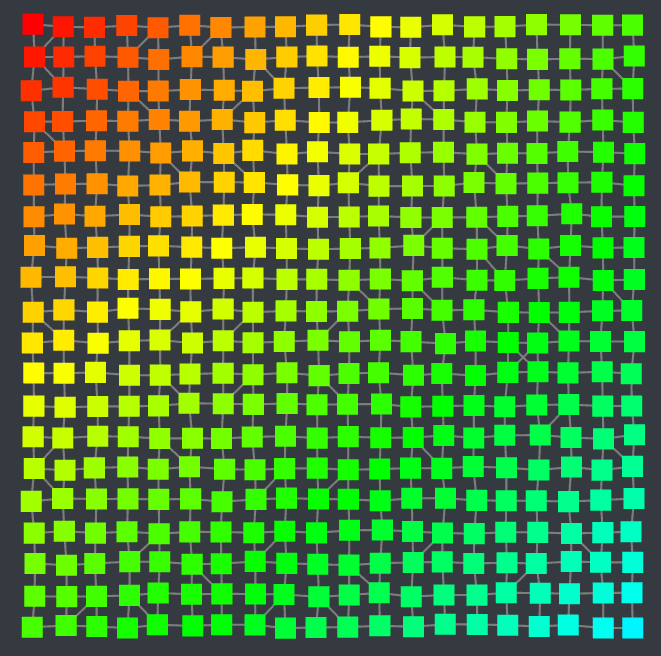
\includegraphics[width=0.5\textwidth]{img/gradient-scafi.png}
      \end{exampleblock}
    \end{column}
  \end{columns}
\end{frame}

\begin{frame}{Future Works}

\end{frame}

\begin{frame}
\centering{
  \Huge{Thank you!}
}
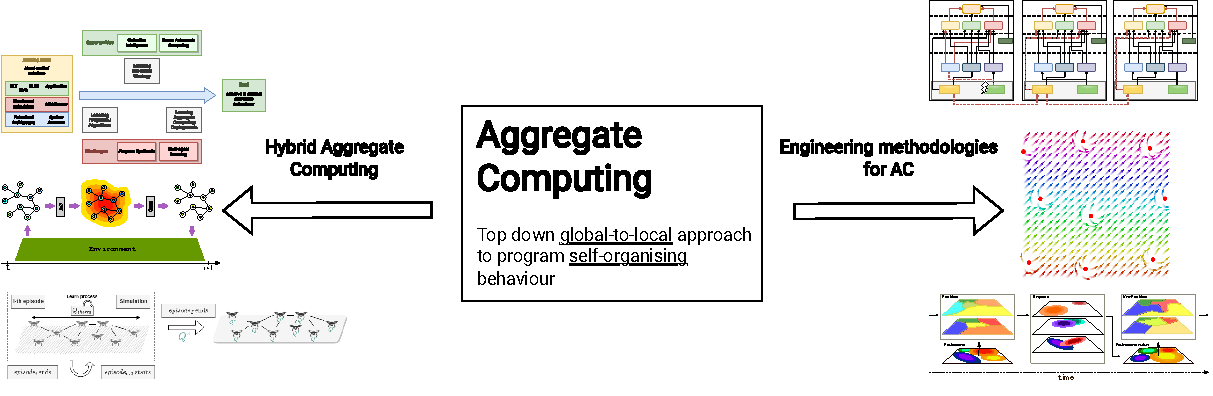
\includegraphics[width=\textwidth]{img/contribution.drawio.pdf}
\end{frame}
\begin{frame}[allowframebreaks]{References}
  \def\bibfont{\footnotesize}
  \printbibliography
\end{frame}

%%%%%%%%%%%%%%%%%%%%%%%%%%%%%%%%%%%%%%%%%%%%%%%%%%%%%%%%%%%%%%%%%%%%%%%%%%%%%%%%
\end{document}
%%%%%%%%%%%%%%%%%%%%%%%%%%%%%%%%%%%%%%%%%%%%%%%%%%%%%%%%%%%%%%%%%%%%%%%%%%%%%%%%
